\documentclass[11pt,a4paper]{article}
\usepackage{better_poster}
\pdfpkresolution=2400
%\pdfimageresolution=2400


% ---- fill in from here

% authors
\title{TERMITE}
\author{H. Deckers, H. Maathuis}

% type of poster: [exp]erimental results, [methods], [theory]
% Disclaimer: the original classification had "study" and "intervention" as separate categories. I group them under experimental results.
\newcommand\postertype{exp} % [exp],[methods],[theory]

\begin{document}

% main point of your study
\makefinding{TERMITE: an interferometer you can build at home}

% the main text of your poster goes here
\makemain{
    % you can have 1 or 2 columns
    \raggedcolumns
    \begin{multicols}{2}
      \section{Goals}
      \begin{itemize}
      \setlength\itemsep{0.1em}
          \item Design and build a Michelson interferometer using readily available lab equipment.
          \item Use this design to measure\\ thermal expansion of samples.
      \end{itemize}

        \section{Design}
        \begin{itemize}
        \setlength\itemsep{0.1em}
            \item Attach one of the mirrors to a sample holder, as it expands or shrinks the pathlength will change and phase-shift the\\ interference pattern.
            \item Measure the temperature and  interference pattern shift as a function of time using a photosensor, thermometer and \\Arduino.
        \end{itemize}


        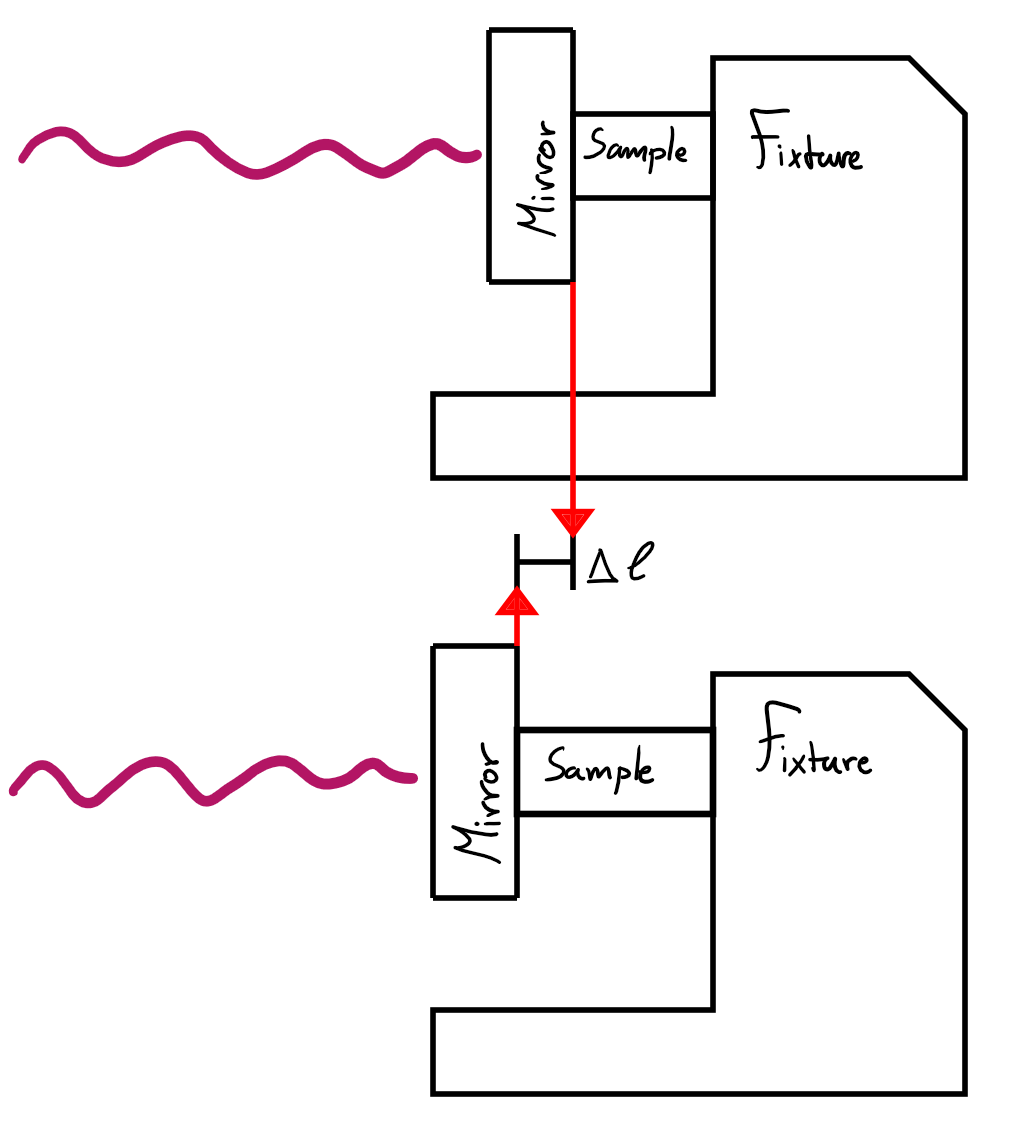
\includegraphics[width=0.9\linewidth]{./images/sample_mirror.png}

    % this determines where your columns will be separated
    \columnbreak

        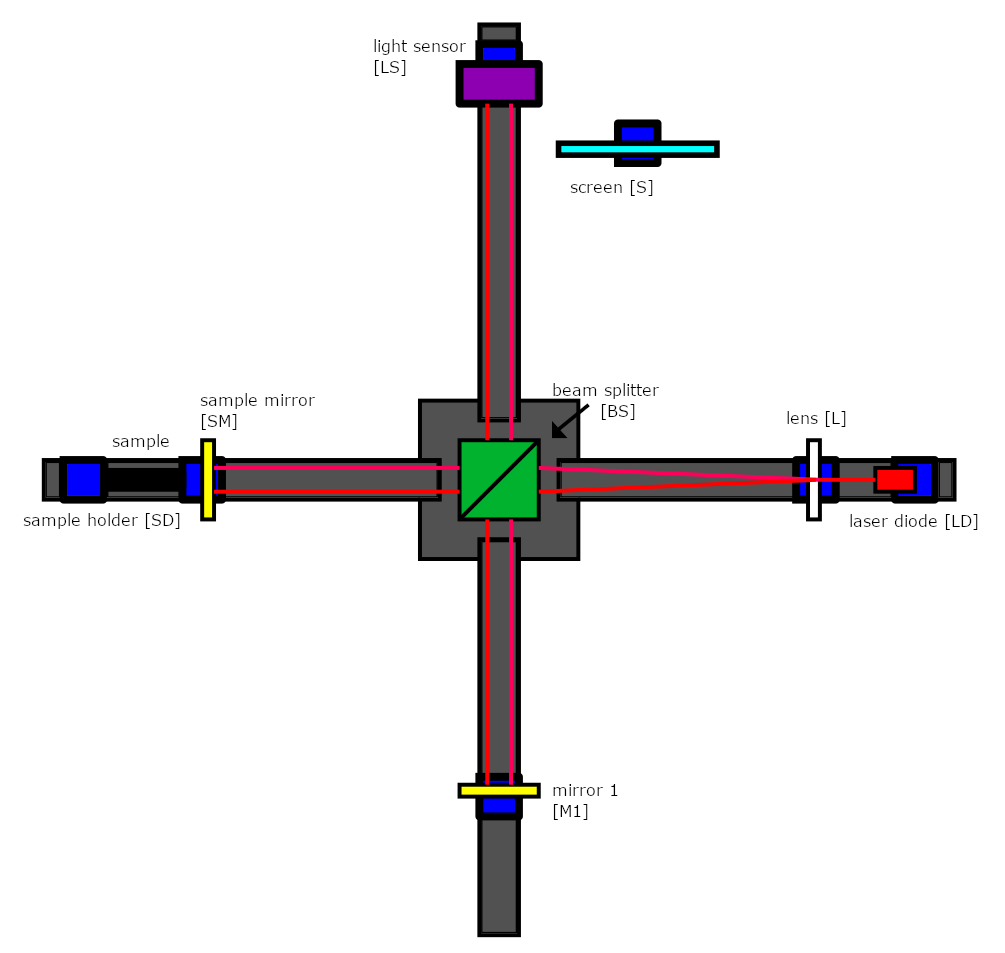
\includegraphics[width=1.1\linewidth]{./images/setup.png}

        \section{Results}
        \begin{itemize}
        \setlength\itemsep{0.1em}
            \item 3D printed interferometer works great, both with and without the sample we saw clear interference patterns!
            \item The sample must be perfectly perpendicular to the laser beam, or the interference pattern will shift out of focus as its temperature changes.
        \end{itemize}

        \section{Conclusion}
        \begin{itemize}
          \setlength\itemsep{0.1em}
            \item Measuring thermal expansion proved difficult due to the alignment issues.
            \item More rigidity and a different light sensor might solve the issues if the project is continued.

        \end{itemize}

    \end{multicols}
}
% If you have extra figures or data to show
\makeextracolumn{
  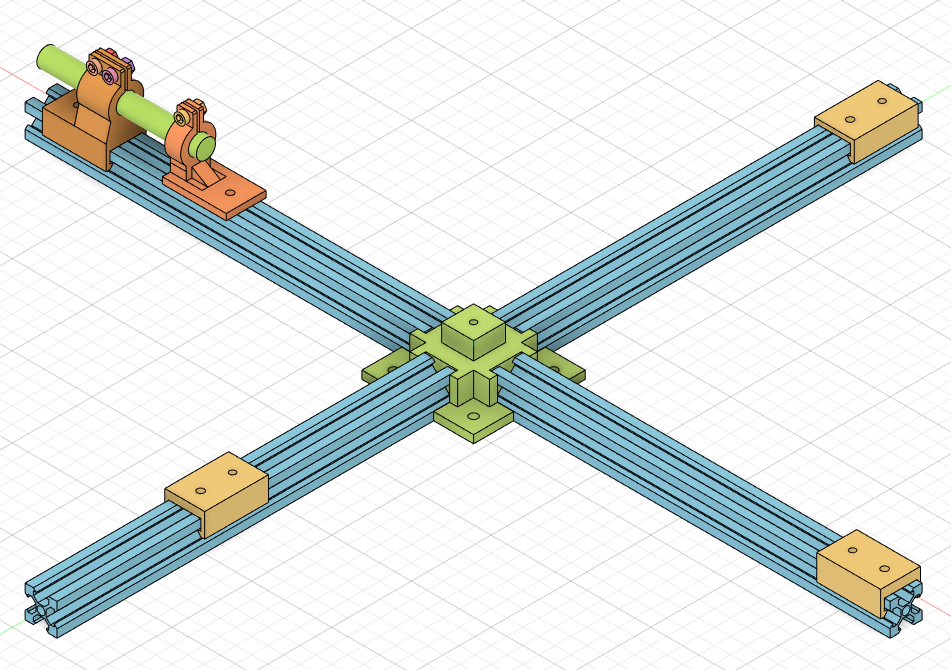
\includegraphics[width=1\linewidth]{./images/design.png}
  Design the experiment in a CAD program!\\
  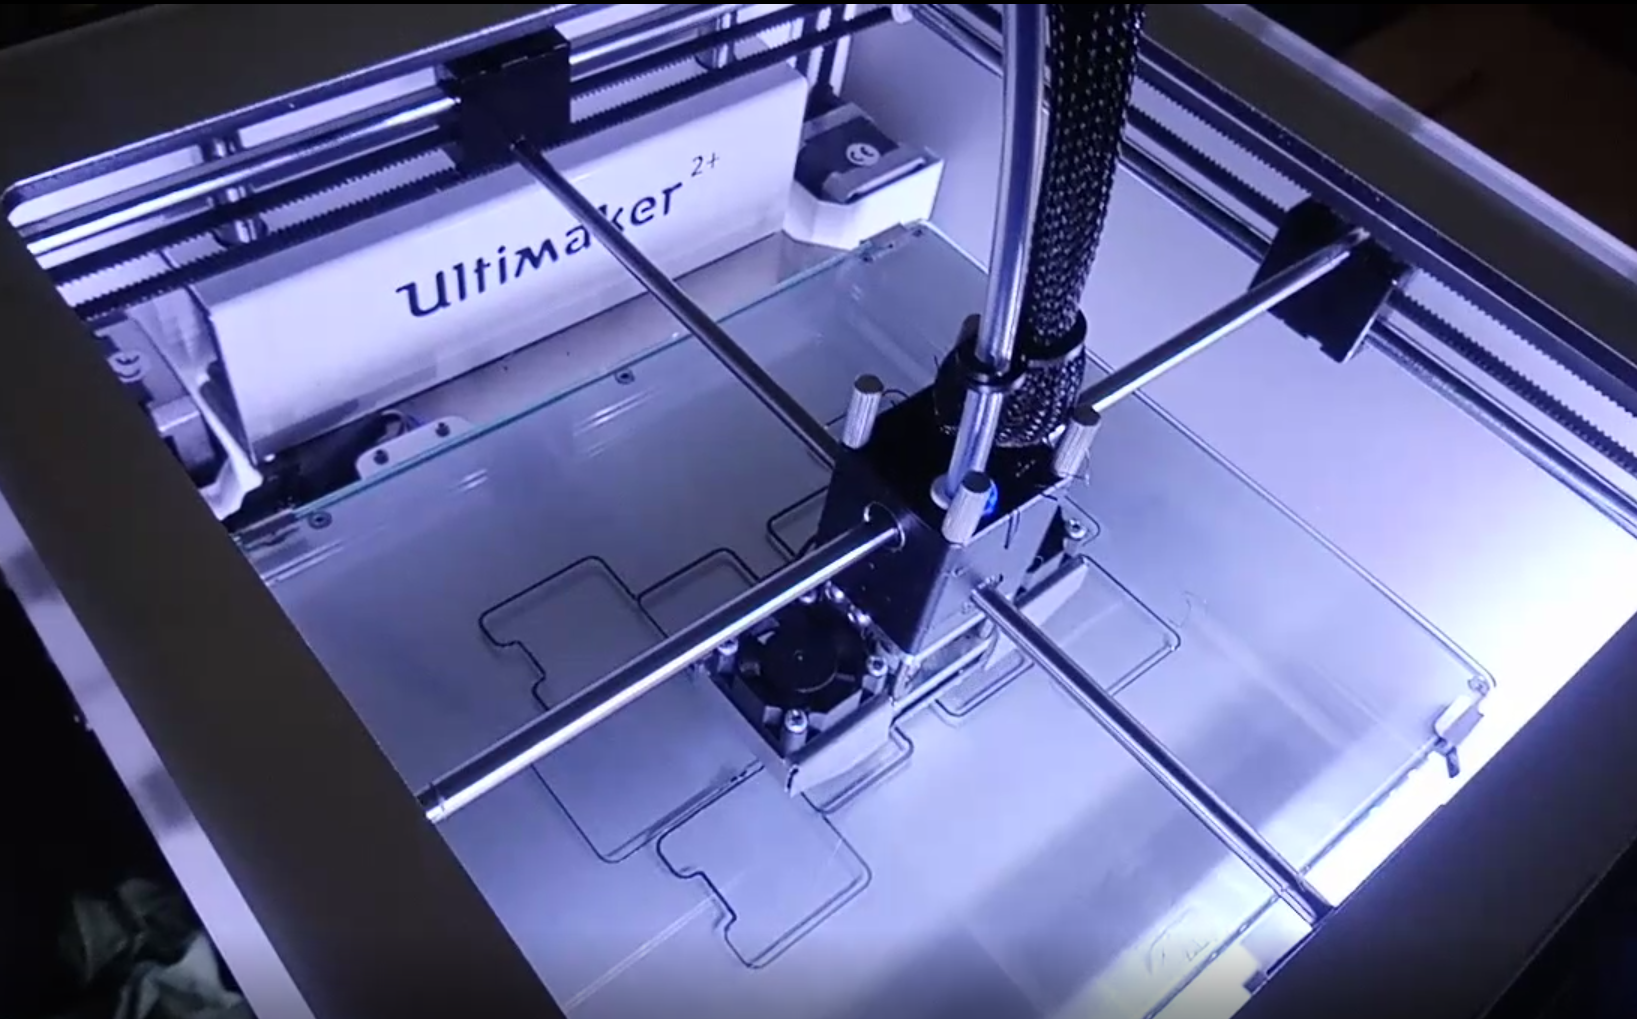
\includegraphics[width=1\linewidth]{./images/print.png}
  Print out the 3D modelled parts,
  source the other parts you need.\\
  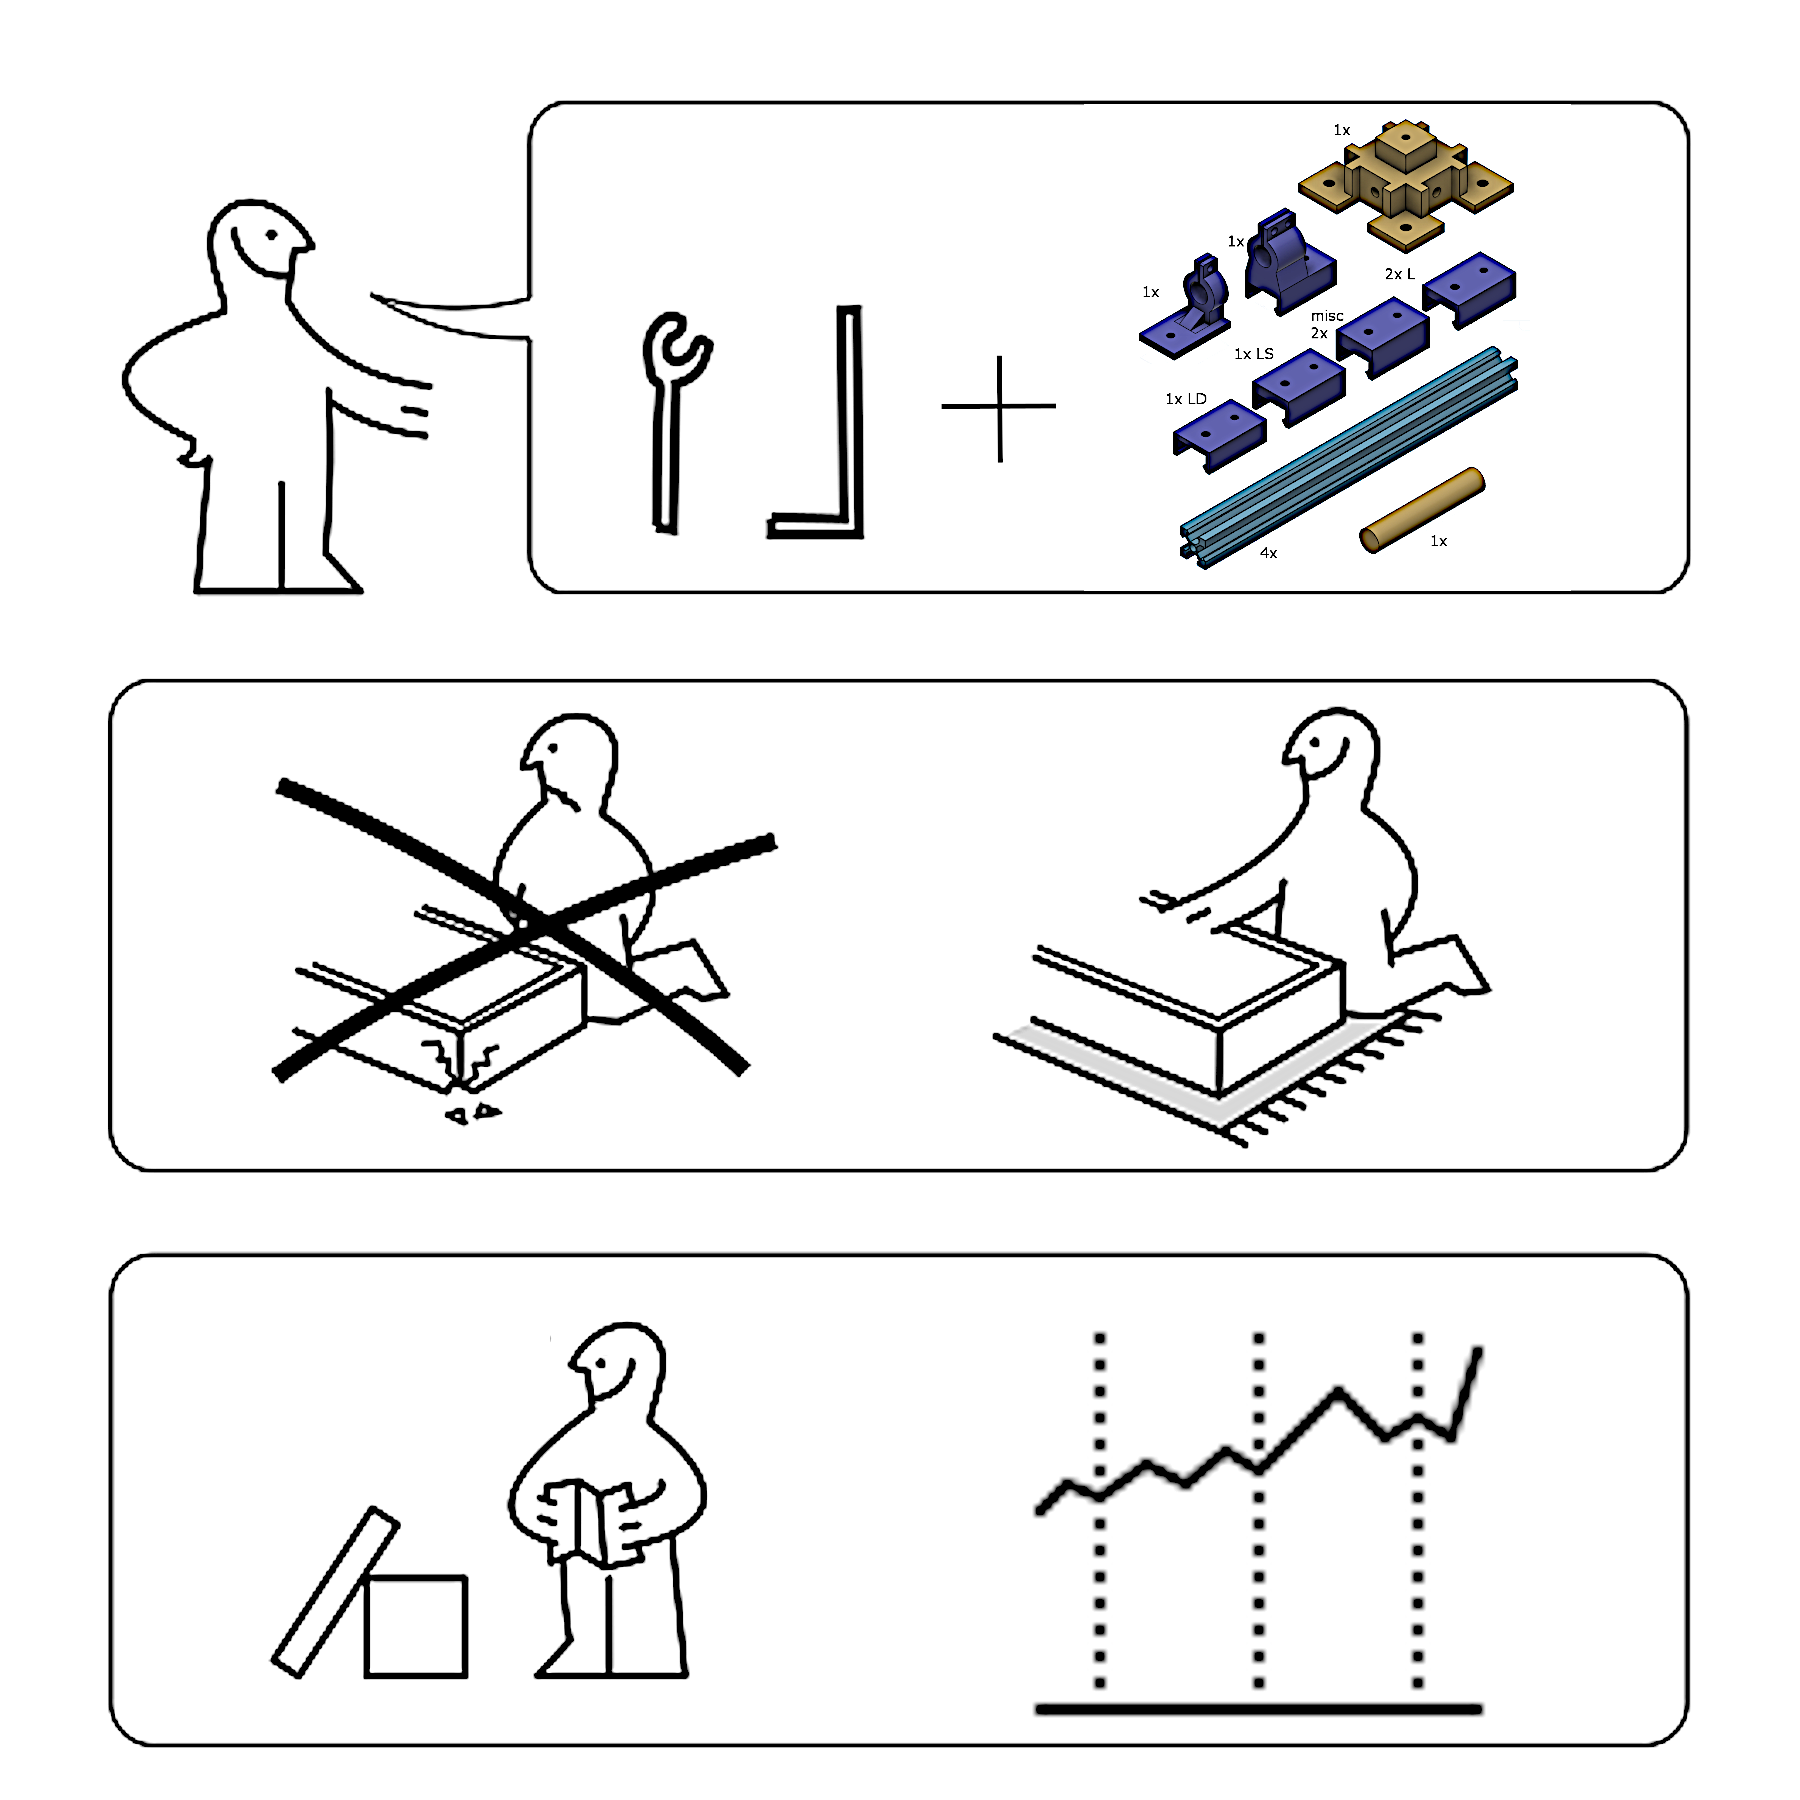
\includegraphics[width=1\linewidth]{./images/build.png}
  Build the setup and try to perform the experiment.\\
  \includegraphics[width=1\linewidth]{./images/experiment.png}

}
% footer
% generate qr code from https://www.qr-code-generator.com/ and replace qr_code.png
% default: barcode on the left
\makefooter{images/uu_logo.png}{images/qr-code.png}

% replace with this like for barcode on the right
%\makealtfooter{images/uni_logo.png}{images/qr-code.png}

\end{document}
